\documentclass{beamer}
%\documentclass[handout]{beamer}
\usepackage[hungarian]{babel}
\uselanguage{hungarian}
\languagepath{hungarian}
\deftranslation[to=hungarian]{Theorem}{T\'etel}
\deftranslation[to=hungarian]{Example}{P\'elda}
\deftranslation[to=hungarian]{Definition}{Defin\'ici\'o}
%\usepackage[magyar]{babel}
\usepackage[utf8]{inputenc}
\usepackage[T1]{fontenc}
\usepackage{listings}
\usepackage{subfig}
\usepackage{xcolor}

\makeatletter
\let\old@lstKV@SwitchCases\lstKV@SwitchCases
\def\lstKV@SwitchCases#1#2#3{}
\makeatother
\usepackage{lstlinebgrd}

\makeatletter
%%%%%%%%%%%%%%%%%%%%%%%%%%%%%%%%%%%%%%%%%%%%%%%%%%%%%%%%%%%%%%%%%%%%%%%%%%%%%%
%
% \btIfInRange{number}{range list}{TRUE}{FALSE}
%
% Test in int number <number> is element of a (comma separated) list of ranges
% (such as: {1,3-5,7,10-12,14}) and processes <TRUE> or <FALSE> respectively

\newcount\bt@rangea
\newcount\bt@rangeb

\newcommand\btIfInRange[2]{%
	\global\let\bt@inrange\@secondoftwo%
	\edef\bt@rangelist{#2}%
	\foreach \range in \bt@rangelist {%
		\afterassignment\bt@getrangeb%
		\bt@rangea=0\range\relax%
		\pgfmathtruncatemacro\result{ ( #1 >= \bt@rangea) && (#1 <= \bt@rangeb) 
		}%
		\ifnum\result=1\relax%
		\breakforeach%
		\global\let\bt@inrange\@firstoftwo%
		\fi%
	}%
	\bt@inrange%
}
\newcommand\bt@getrangeb{%
	\@ifnextchar\relax%
	{\bt@rangeb=\bt@rangea}%
	{\@getrangeb}%
}
\def\@getrangeb-#1\relax{%
	\ifx\relax#1\relax%
	\bt@rangeb=100000%   \maxdimen is too large for pgfmath
	\else%
	\bt@rangeb=#1\relax%
	\fi%
}

%%%%%%%%%%%%%%%%%%%%%%%%%%%%%%%%%%%%%%%%%%%%%%%%%%%%%%%%%%%%%%%%%%%%%%%%%%%%%%
%
% \btLstHL<overlay spec>{range list}
%
% TODO BUG: \btLstHL commands can not yet be accumulated if more than one 
%overlay spec match.
% 
\newcommand<>{\btLstHL}[1]{%
	\only#2{\btIfInRange{\value{lstnumber}}{#1}{\color{orange!30}\def\lst@linebgrdcmd{\color@block}}{\def\lst@linebgrdcmd####1####2####3{}}}%
}%
\makeatother



\usepackage{hyperref}
\hypersetup{
    colorlinks = true,
    linkcolor = blue,
    urlcolor  = blue,
    citecolor = blue,
    linkbordercolor = {white},
}
\usepackage{tikz}
\usetikzlibrary{trees}
\usetikzlibrary{shapes,shapes.geometric,shapes.multipart}
\usetikzlibrary{calc,chains,arrows,positioning}
\tikzset{
  bnode/.style={rectangle split, rectangle split parts=3, rectangle split horizontal,rectangle split ignore empty parts,draw, fill=white},
  box/.style={draw, fill=pink!10, minimum width=5em, text centered, minimum height=2.5em},
  treenode/.style = {align=center, inner sep=0pt, text centered, font=\sffamily},
  arn_n/.style = {treenode, circle, white, font=\sffamily\bfseries, draw=black, fill=black, text width=1.5em},
  arn_r/.style = {treenode, circle, red, draw=red, text width=1.5em, very thick}
}
\usetheme{Warsaw}
\institute{Szegedi Tudományegyetem}
\pgfdeclareimage[height=0.55cm]{institution-logo}{../szte_logo}
\logo{\pgfuseimage{institution-logo}}

\title{Algoritmusok és adatszerkezetek II.}
\subtitle{2-3-4 fák és piros-fekete fák}
\date{}

\begin{document}

\maketitle

\begin{frame}{Szolgálati közlemény}
\begin{alertblock}{Emlékeztető}
Már kitölthető az első Coospace kvíz. \\
\end{alertblock}

\begin{block}{Egyebek}
\begin{itemize}
\item Hallgatói ösztöndíjlehetőség a mestint tanszéken
\item 
\href{https://github.com/begab/alga2/blob/master/szorgalmi/feladatok.pdf}{Szorgalmi
 feladatok}
\item 
\href{https://docs.google.com/forms/d/e/1FAIpQLSdudmDtFcVYwumCu3s90kJh_oDMKvTtFUhVwCqvZclGSjw6vw/viewform?usp=sf_link}{Értékelés}
\end{itemize}
\end{block}
\end{frame}

\begin{frame}{2-3-4 fa}
	\begin{block}{Definíció}
	2-3-4 fa alatt olyan \textbf{általános keresőfát} értünk, amelynek minden 
	$x$ csúcsára $Rang(x) \in \{1,2,3\}$ \hfill {\tiny (Mégis miért hívjuk 
	akkor 2-3-4 fának?)}
	\end{block}
	
	\begin{example}
			\begin{figure}
				\centering
				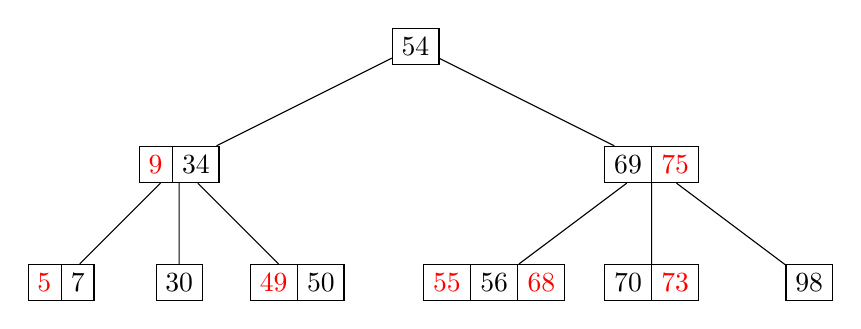
\begin{tikzpicture}
					\tikzstyle{every node}=[bnode]
					\node {54}
						child[sibling distance=6cm] {node{\color{red}{9} 
						\nodepart{two} 34}
							child[sibling distance=1.5cm]{node{\color{red}{5} 
							\nodepart{two} 7}}
							child[sibling distance=1.5cm]{node{30}}
							child[sibling distance=1.5cm]{node{\color{red}{49} 
							\nodepart{two} 50}}
						}
						child[sibling distance=6cm] {node{69 \nodepart{two} 
						\color{red}{75}}
							child[sibling distance=2cm]{node{\color{red}55 
							\nodepart{two} 56 \nodepart{three} \color{red}68}}
							child[sibling distance=1.5cm]{node{70 
							\nodepart{two} \color{red}{73}}}
							child[sibling distance=2cm]{node{98}}
						};
				\end{tikzpicture}
			\end{figure}
	\end{example}
\end{frame}

\begin{frame}{Piros-fekete fák tulajdonságai}
	\begin{enumerate}
		\item Minden csúcs színe piros vagy fekete
		\item A gyökér színe fekete
		\item Minden levele\footnote{levelek alatt itt most az ''őrszemeket'' 
		értjük} fekete
		\item A piros csúcsoknak \textbf{kizárólag} fekete színű gyerekeik 
		vannak
		\item Bármely csúcsból azonos számú fekete csúcs érintésével jutunk el 
		bármelyik levélbe
	\end{enumerate}

	\pause
	\begin{theorem}
		Bármely $n$ kulcsú piros-fekete fa magassága legfeljebb $2\log(n+1)$.
	\end{theorem}
\end{frame}

\begin{frame}{Fekete-magasság}
	\begin{itemize}
		\item $bh(x)$ jelölje az $x$ csúcsból induló, bármely levélig vezető 
		úton található,
		($x$-en kívüli) fekete csúcsok számát
	\end{itemize}
	\begin{columns}
		\begin{column}{0.4\linewidth}
			\begin{example}
				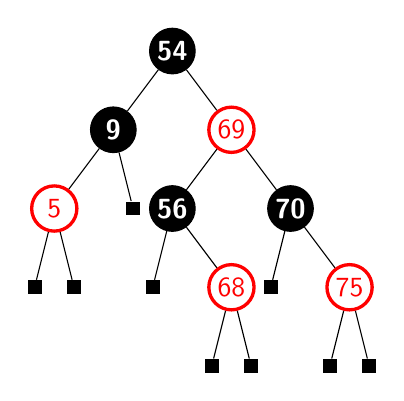
\begin{tikzpicture}[level distance=1cm]
				\node [arn_n] {54}
					child{ node [arn_n] {9}
						child{ node [arn_r] {5}
							child[sibling distance=0.5cm]{ 
							node[fill=black,inner sep=0pt,minimum size=5pt] {}}
							child[sibling distance=0.5cm]{ 
							node[fill=black,inner sep=0pt,minimum size=5pt] {}}
						}
						child[sibling distance=0.5cm]{ node[fill=black,inner 
						sep=0pt,minimum size=5pt] {}}
					}
					child{ node [arn_r] {69}
						child{ node [arn_n]  {56}
							child[sibling distance=0.5cm]{ 
							node[fill=black,inner sep=0pt,minimum size=5pt] {}}
							child{ node [arn_r]  {68}
								child[sibling distance=0.5cm]{ 
								node[fill=black,inner sep=0pt,minimum size=5pt] 
								{}}
								child[sibling distance=0.5cm]{ 
								node[fill=black,inner sep=0pt,minimum size=5pt] 
								{}}
							}
						}
						child{ node [arn_n]  {70}
							child[sibling distance=0.5cm]{ 
							node[fill=black,inner sep=0pt,minimum size=5pt] {}}
							child{ node [arn_r]  {75}
								child[sibling distance=0.5cm]{ 
								node[fill=black,inner sep=0pt,minimum size=5pt] 
								{}}
								child[sibling distance=0.5cm]{ 
								node[fill=black,inner sep=0pt,minimum size=5pt] 
								{}}
							}
						}
					};
				\end{tikzpicture}
			\end{example}
		\end{column}
		\begin{column}{0.6\linewidth}
			\begin{block}<2>{}
			 A (teljes) fa fekete-magassága 2 \\
 			 A 9 gyökerű fa fekete-magassága 1 \\
 			 A 69 gyökerű fa fekete-magassága 2 \\
			\end{block}
		\end{column}
	\end{columns}
\end{frame}

\begin{frame}{A piros-fekete fák legrosszabb magasságának igazolása}
	\begin{alertblock}{Fontos észrevételek}
		\begin{enumerate}	
		\item $x$ gyökerű fa $h(x)$ magassága $\geq bh(x)$
		\item $x$ minden $y$ gyerekére $bh(y)=bh(x)$ vagy $bh(y)=bh(x)-1$
		\item $x$ minden $y$ gyerekére $h(y) \leq h(x)-1$
		\end{enumerate}
	\end{alertblock}
	
	\begin{block}<2->{Minden $x$ gyökerű fa legalább $2^{bh(x)}-1$ csúcsot 
	tartalmaz.}
		0 magas fára természetesen teljesül. \\
		Az $x$ gyökerű fában legalább annyi csúcs van, mint ahány csúcs a 
		fiaiban legalább van + 1, azaz $2*(2^{bh(x)-1}-1)+1=2^{bh(x)}-1$
	\end{block}
	
	\begin{block}<3->{A piros-fekete fák 4. tulajdonságából következően}
	 Bármely $x$-ből levélig menő úton az érintett csúcsok \textbf{legalább} 
	 1/2-e fekete \pause $\Rightarrow bh(x) \geq h(x)/2$, vagyis az $x$ gyökerű 
	 fában lévő $n$ kulcsok száma $n \geq 2^{h/2}-1$ \pause $\Rightarrow h \leq 
	 2 \log (n+1) $
	\end{block}
\end{frame}

\begin{frame}[fragile]{Piros-fekete fa implementációja}
	\begin{columns}
		\begin{column}{.6\textwidth}
\begin{lstlisting}[
  linebackgroundcolor={
    \btLstHL<1->{3}
  }]
class Node {
    Object kulcs;
    boolean fekete;
    Node *apa;
    Node *bal;
    Node *jobb;
}
\end{lstlisting}
			\begin{block}<2>{Megjegyzés}
				Csupán 1 bitnyi kiegészítő információ\\
				$\Rightarrow$ akár a kulcsba is integrálható
			\end{block}
		\end{column}
		
		\begin{column}{.4\textwidth}
		\begin{figure}
		\centering
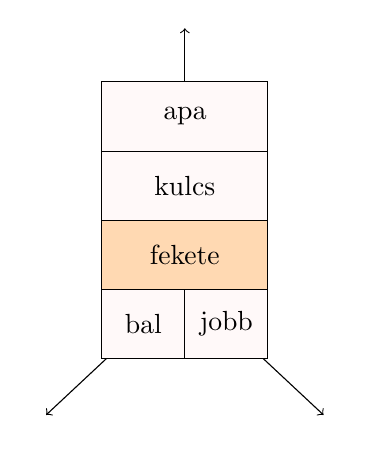
\begin{tikzpicture}[node distance=0cm,outer sep = 0pt]
    \node (A) [box,minimum width=6em] {kulcs};
    \node (H) [box,anchor=north,minimum width=6em,fill=orange!30] at (A.south) 
    {fekete};
    \node (D) [box,anchor=south,minimum width=6em] at (A.north) {apa};
    \node (B) [box,anchor=north west,minimum width=3em] at (H.south west) {bal};
    \node (C) [box,anchor=north east,minimum width=3em] at (H.south east) 
    {jobb};
    \coordinate (E) at (0,2);
    \coordinate (E) at (0,2);
    \node[below left = 1cm of B] (F) {};
    \node[below right = 1cm of C] (G) {};
%    \path (D) edge [->] node[pos=0.5,anchor=-135,inner sep=1pt] {N} (E);
    \path (D) edge [->] (E);
    \path (B) edge [->] (F);
    \path (C) edge [->] (G);
\end{tikzpicture}
		\end{figure}
		\end{column}
	\end{columns}
\end{frame}

\begin{frame}{AVL vs. piros-fekete fa}
	\begin{block}{AVL fa legrosszabb magassága jobb, mint a piros-fekete fáé}
        $h < 1.45*h_{OTP}(n)$ \hfill vs. \hfill $h \leq 2*h_{OPT}(n)$
		\begin{itemize}
			\item $h_{OPT}(n)$ az $n$ kulcsot tartalmazó, teljesen 
			kiegyensúlyozott bináris keresőfa magassága
			\item<2-> Gyakorlati jelentősége minimális: $n=2^{30}-1 > 10^9$-ra 
			azt kapjuk, hogy egy AVL/piros-fekete-fa legfeljebb 44/60 magas
			\item<2-> Ha a {\scshape Keres} művelet végrehajtása dominál, el 
			lehet gondolkozni az AVL-fa használatán
		\end{itemize}
	\end{block}
	\begin{alertblock}<3>{}
		\begin{itemize}
			\item A {\scshape{Beszúr}} és {\scshape{Töröl}} műveletek 
			ugyanakkor implementációs szempontból 
			\href{https://stackoverflow.com/questions/13852870/red-black-tree-over-avl-tree}{egyszerűbbek/gyorsabbak
			 piros-fekete fákra}
		\end{itemize}
	\end{alertblock}
\end{frame}

\begin{frame}{A helyreállítás (egyik) záloga -- átszínezés}
	\begin{itemize}
		\item Ha van egy valid piros-fekete fánk, amelynek egy $x$ csúcsa 
		fekete, fiai viszont pirosak, akkor az 5.~tulajdonságot nem sértő fát 
		kapunk akkor is, ha $x$ pirosra, fiai pedig feketére váltanak
		\item Másképpen, ha piros testvérpár színe feketére vált, a közös 
		szülőnek a továbbiakban nem kell feketének lennie
	\end{itemize}
	
		\begin{columns}
			\begin{column}{0.5\linewidth}
				\begin{figure}
				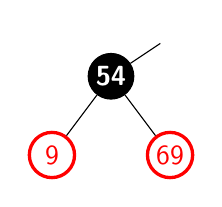
\begin{tikzpicture}
				\node[draw=none] {}
				 child[level distance=0.5cm]{ node [arn_n] {54}
					child[level distance=1cm]{ node [arn_r] {9}}
					child[level distance=1cm]{ node [arn_r] {69}}
					}
					child[missing];
				\end{tikzpicture}
				\end{figure}
			\end{column}
			\begin{column}{0.5\linewidth}
				\begin{figure}
				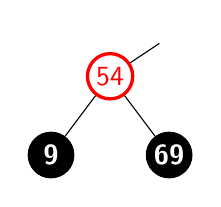
\begin{tikzpicture}
				\node[draw=none] {}
				 child[level distance=0.5cm]{ node [arn_r] {54}
					child[level distance=1cm]{ node [arn_n] {9}}
					child[level distance=1cm]{ node [arn_n] {69}}
					}
					child[missing];
				\end{tikzpicture}
				\end{figure}
			\end{column}
		\end{columns}
\end{frame}

\begin{frame}{Beszúrás utáni javítás átszínezéssel}
	\begin{itemize}
		\item A beszúrandó kulcsot piros színnel szúrjuk be (arra a helyre 
		ahova egyébként egy bináris keresőfába tennénk)
		\item Mitől romolhat el beszúrás kapcsán a piros-fekete fa?
		\begin{itemize}
			\item<2-> Ha piros szülő jut piros gyerekhez
		\end{itemize}
	\end{itemize}
	\begin{columns}
		\begin{column}<2->{0.5\linewidth}
			\begin{figure}
			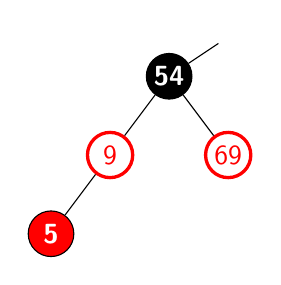
\begin{tikzpicture}
			\node[draw=none] {}
			 child[level distance=0.5cm]{ node [arn_n] {54}
				child[level distance=1cm]{ node [arn_r] {9}
					child{ node [treenode, circle, white, 
					font=\sffamily\bfseries, draw=black, fill=red, text 
					width=1.5em] {5}}
					child[missing]
				}
				child[level distance=1cm]{ node [arn_r] {69}}
				}
				child[missing];
			\end{tikzpicture}
			\end{figure}
		\end{column}
		\begin{column}<3>{0.5\linewidth}
			\begin{figure}
			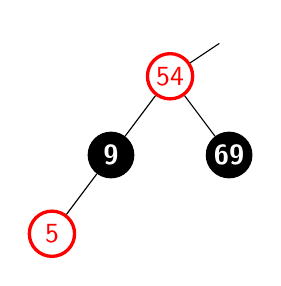
\begin{tikzpicture}
			\node[draw=none] {}
			 child[level distance=0.5cm]{ node [arn_r] {54}
				child[level distance=1cm]{ node [arn_n] {9}
					child{ node [arn_r] {5}}
					child[missing]
				}
				child[level distance=1cm]{ node [arn_n] {69}}
				}
				child[missing];
			\end{tikzpicture}
			\end{figure}
		\end{column}
	\end{columns}
	\begin{block}<3>{Mi lehet ennek a helyreállításnak a velejárója?}
	A pirosra színezett csúcs mentén újabb helyreállításra lehet szükség
	\end{block}	
\end{frame}

\begin{frame}{Beszúrás utáni javítás forgatással}
	\begin{itemize}
		\item $\alpha, \beta, \gamma, \delta$ egy-egy részfát jelöl
		\item Az előző helyzettől az különbözteti meg a mostanit, hogy a 
		beszúrt kulcs nagybátyja (a $\delta$ részfa gyökere) fekete
		\item AVL fákhoz hasonlóan, itt is a ''cikk-cakkos'' esetben van 
		szükség 2 forgatásra (a cikk-cakkot $\delta$-hoz viszonyítva nézzük)
	\end{itemize}
	\begin{figure}
		\subfloat[2 forgatás kell]{
			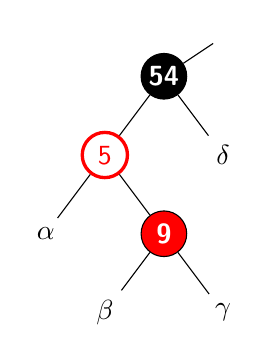
\begin{tikzpicture}
			\node[draw=none] {}
			 child[level distance=.5cm]{ node [arn_n] {54}
				child[level distance=1cm]{ node [arn_r] {5}
					child {node {$\alpha$}}
					child{ node [treenode, circle, white, 
					font=\sffamily\bfseries, draw=black, fill=red, text 
					width=1.5em] {9}
						child {node {$\beta$}}
						child {node {$\gamma$}}
					}
				}
				child[level distance=1cm]{ node [] {$\delta$}}
				}
			child[missing];
			\end{tikzpicture}
		} ~
		\subfloat[1 forgatás elég]{
			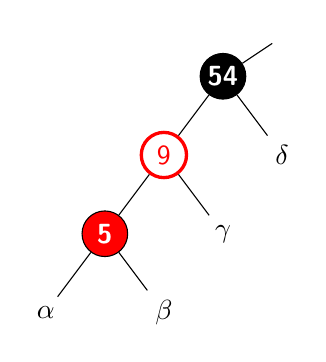
\begin{tikzpicture}
			\node[draw=none] {}
			 child[level distance=.5cm]{ node [arn_n] {54}
				child[level distance=1cm]{ node [arn_r] {9}
					child{ node [treenode, circle, white, 
					font=\sffamily\bfseries, draw=black, fill=red, text 
					width=1.5em] {5}
						child {node {$\alpha$}}
						child {node {$\beta$}}
					}
					child {node {$\gamma$}}
				}
				child[level distance=1cm]{ node [] {$\delta$}}
				}
			child[missing];
			\end{tikzpicture}
		}~
		\subfloat[helyreállítás után]{
			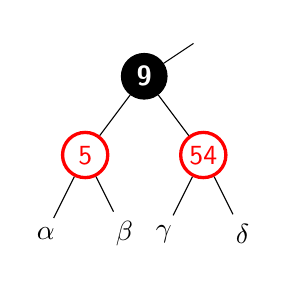
\begin{tikzpicture}
			\node[draw=none] {}
			 child[level distance=.5cm]{ node [arn_n] {9}
					child[level distance=1cm]{ node [arn_r] {5}
						child[sibling distance=1cm] {node {$\alpha$}}
						child[sibling distance=1cm] {node {$\beta$}}
					}
					child[level distance=1cm]{ node [arn_r] {54}
						child[sibling distance=1cm] {node {$\gamma$}}
						child[sibling distance=1cm] {node {$\delta$}}
					}
				}
				child[missing];
		\end{tikzpicture}
		}
	\end{figure}
\end{frame}

\begin{frame}{Törlés utáni javítás átszínezéssel}
	\begin{itemize}
		\item Bajt az okozhat, ha kiesik egy fekete csúcs
		\item A kieső csúcs feketeségét át kell ruházni, hiszen két 
		''rétegnyi'' feketeségért semelyik csúcs sem lehet felelős
		\item Ha a duplán fekete csúcs testvére és unokaöccsei is feketék, a 
		szülő át tudja vállalni a feketeséget
	\end{itemize}
	\begin{columns}
		\begin{column}{0.5\linewidth}
			\begin{figure}
			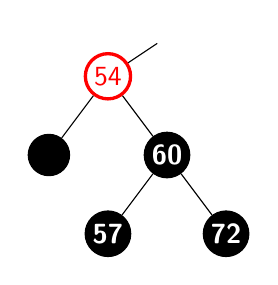
\begin{tikzpicture}
			\node[draw=none]{}
			 	child[level distance=0.5cm]{ node [arn_r] {54}
					child[level distance=1cm]{ node [arn_n] {}}
					child[level distance=1cm]{ node [arn_n] {60}
						child[level distance=1cm]{ node [arn_n] {57}}
						child[level distance=1cm]{ node [arn_n] {72}}
					}
				}
				child[missing];
			\end{tikzpicture}
			\end{figure}
		\end{column}
		\begin{column}<2->{0.5\linewidth}
			\begin{figure}
			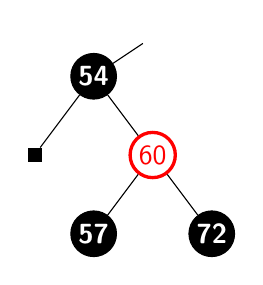
\begin{tikzpicture}
			\node[draw=none]{}
			 	child[level distance=0.5cm]{ node [arn_n] {54}
					child[sibling distance=1.5cm, level distance=1cm]{ 
					node[fill=black,inner sep=0pt,minimum size=5pt] {}}
					child[level distance=1cm]{ node [arn_r] {60}
						child[level distance=1cm]{ node [arn_n] {57}}
						child[level distance=1cm]{ node [arn_n] {72}}
					}
				}
				child[missing];
			\end{tikzpicture}
			\end{figure}
		\end{column}
	\end{columns}
	\begin{block}<3>{Mi történt volna, ha a duplán fekete csúcs apja nem piros?}
	Szükség esetén a helyreállítást az apától folytathatjuk tovább.
	\end{block}	
\end{frame}

\begin{frame}{Törlés utáni javítás forgatással}
	\begin{itemize}
		\item Piros unokaöcs esetén forgatásra van szükség
		\item Ha a ($d$-vel megjelölt) duplán fekete csúcs távolabbi unokaöccse 
		(E) piros, 1 forgatás is elég
		\item<2> Valóban, az egyes részfákig a forgatást követően is ugyanannyi 
		fekete csúcs érintésével tudunk eljutni
		\begin{itemize}
			\item $\alpha$ és $\beta$: 2/3; $\gamma$, $\epsilon$ és $\zeta$: 
			1/2 (B kezdeti színétől függően)
		\end{itemize}
	\end{itemize}
	\begin{figure}
		\subfloat[helyreállítás előtt]{
			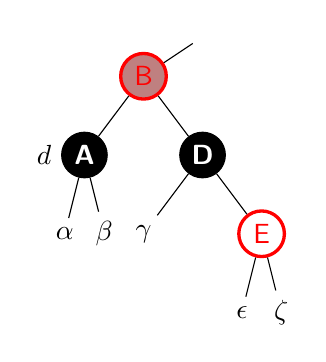
\begin{tikzpicture}
			\node[draw=none]{}
			 	child[level distance=0.5cm]{ node [arn_r,fill=black!50!red!50] 
			 	{B}
			 		child[level distance=1cm]{ node [label={left:$d$},arn_n] {A}
						child[sibling distance=.5cm] {node {$\alpha$}}
						child[sibling distance=.5cm] {node {$\beta$}}
					}
					child[level distance=1cm]{ node [arn_n] {D}
						child[level distance=1cm]{ node {$\gamma$}}
						child[level distance=1cm]{ node [arn_r] {E}
							child[sibling distance=.5cm] {node {$\epsilon$}}
							child[sibling distance=.5cm] {node {$\zeta$}}
						}
					}
				}
				child[missing];
			\end{tikzpicture}
		} \hfill
		\only<2>{
		\subfloat[helyreállítás után]{
			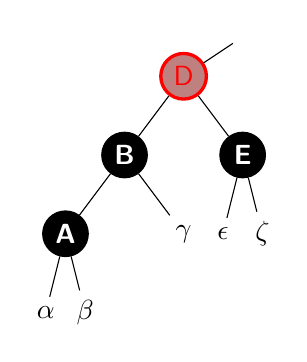
\begin{tikzpicture}
			\node[draw=none]{}
			 	child[level distance=0.5cm]{ node [arn_r,fill=black!50!red!50] 
			 	{D}
			 		child[level distance=1cm]{ node [arn_n] {B}
				 		child[level distance=1cm]{ node [arn_n] {A}
							child[sibling distance=.5cm] {node {$\alpha$}}
							child[sibling distance=.5cm] {node {$\beta$}}
						}
						child[level distance=1cm]{ node {$\gamma$}}
					}
					child[level distance=1cm]{ node [arn_n] {E}
						child[sibling distance=.5cm] {node {$\epsilon$}}
						child[sibling distance=.5cm] {node {$\zeta$}}
					}
				}
				child[missing];
			\end{tikzpicture}
		}}
	\end{figure}
\end{frame}

\begin{frame}{Törlés utáni javítás segédforgatással}
	\begin{itemize}
		\item Piros unokaöcs esetén forgatásra van szükség
		\item Ha a ($d$-vel megjelölt) duplán fekete csúcs távolabbi unokaöccse 
		fekete (de a közelebbi nem), segédforgatunk
		\item<2> 1 további forgatással garantáltan orvosolható (hiszen a duplán 
		fekete csúcs távolabbi unokaöccse piros lett, lásd előző eset)
	\end{itemize}
	\begin{figure}
		\subfloat[segédforgatás előtt]{
			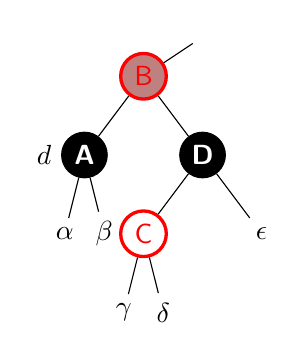
\begin{tikzpicture}
			\node[draw=none]{}
			 	child[level distance=0.5cm]{ node [arn_r,fill=black!50!red!50] 
			 	{B}
			 		child[level distance=1cm]{ node [label={left:$d$},arn_n] {A}
						child[sibling distance=.5cm] {node {$\alpha$}}
						child[sibling distance=.5cm] {node {$\beta$}}
					}
					child[level distance=1cm]{ node [arn_n] {D}
						child[level distance=1cm]{ node [arn_r] {C}
							child[sibling distance=.5cm] {node {$\gamma$}}
							child[sibling distance=.5cm] {node {$\delta$}}
						}
						child[level distance=1cm]{ node {$\epsilon$}}
					}
				}
				child[missing];
			\end{tikzpicture}
		} \hfill
		\only<2>{
		\subfloat[segédforgatás után]{
			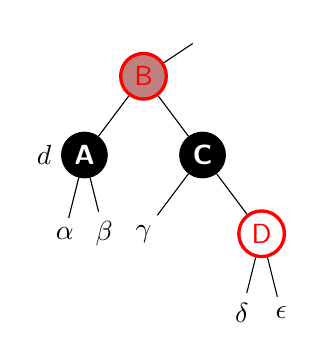
\begin{tikzpicture}
			\node[draw=none]{}
			 	child[level distance=0.5cm]{ node [arn_r,fill=black!50!red!50] 
			 	{B}
			 		child[level distance=1cm]{ node [label={left:$d$},arn_n] {A}
						child[sibling distance=.5cm] {node {$\alpha$}}
						child[sibling distance=.5cm] {node {$\beta$}}
					}
					child[level distance=1cm]{ node [arn_n] {C}
						child[level distance=1cm]{ node {$\gamma$}}
						child[level distance=1cm]{ node [arn_r] {D}
							child[sibling distance=.5cm] {node {$\delta$}}
							child[sibling distance=.5cm] {node {$\epsilon$}}
						}
					}
				}
				child[missing];
			\end{tikzpicture}
			}
		}
	\end{figure}
\end{frame}

\begin{frame}{Egy további eshetőség segédforgatásra}
	\begin{itemize}
		\item Piros testvér esetén is forgatni kell
		\item<2> A duplán fekete csúcs megmarad, de a forgatást követően 
		biztosan valamelyik már tárgyalt eset áll elő
	\end{itemize}
	\begin{figure}
		\subfloat[segédforgatás előtt]{
			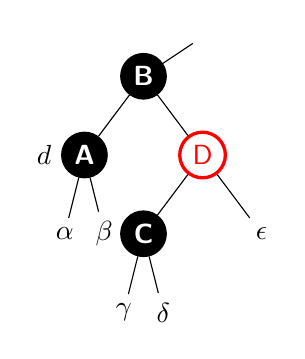
\begin{tikzpicture}
			\node[draw=none]{}
			 	child[level distance=0.5cm]{ node [arn_n] {B}
			 		child[level distance=1cm]{ node [label={left:$d$},arn_n] {A}
						child[sibling distance=.5cm] {node {$\alpha$}}
						child[sibling distance=.5cm] {node {$\beta$}}
					}
					child[level distance=1cm]{ node [arn_r] {D}
						child[level distance=1cm]{ node [arn_n] {C}
							child[sibling distance=.5cm] {node {$\gamma$}}
							child[sibling distance=.5cm] {node {$\delta$}}
						}
						child[level distance=1cm]{ node {$\epsilon$}}
					}
				}
				child[missing];
			\end{tikzpicture}
		} \hfill
		\only<2>{
		\subfloat[segédforgatás után]{
			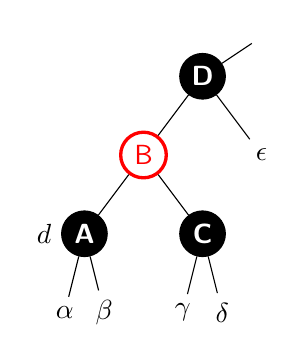
\begin{tikzpicture}
			\node[draw=none]{}
			 	child[level distance=0.5cm]{ node [arn_n] {D}
			 		child[level distance=1cm]{ node [arn_r] {B}
				 		child[level distance=1cm]{ node 
				 		[label={left:$d$},arn_n] {A}
							child[sibling distance=.5cm] {node {$\alpha$}}
							child[sibling distance=.5cm] {node {$\beta$}}
						}
				 		child[level distance=1cm]{ node [arn_n] {C}
							child[sibling distance=.5cm] {node {$\gamma$}}
							child[sibling distance=.5cm] {node {$\delta$}}
						}
					}
					child[level distance=1cm]{ node {$\epsilon$}}
				}
				child[missing];
			\end{tikzpicture}
		}}
	\end{figure}
\end{frame}

\begin{frame}{2-3-4 és piros-fekete fák közötti kapcsolat}
	\begin{figure}
	\begin{minipage}[c]{.4\textwidth}
		\subfloat{
			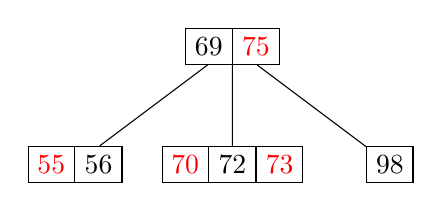
\begin{tikzpicture}
				\tikzstyle{every node}=[bnode]
				\node {69 \nodepart{two} \color{red}{75}}
				child[sibling distance=2cm]{
					node{\color{red}55 \nodepart{two} 56 }}
				child[sibling distance=2cm]{
					node{\color{red}{70} \nodepart{two} 72 \nodepart{three} 
					\color{red}{73}}}
				child[sibling distance=2cm]{node{98}};
			\end{tikzpicture}
		}
		\end{minipage}
		 \hfill
		\begin{minipage}[c]{.4\textwidth}
		\subfloat{
			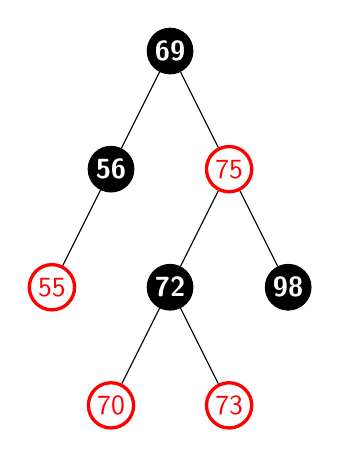
\begin{tikzpicture}
	\node [arn_n] {69}
			child{ node [arn_n]  {56}
				child{ node [arn_r] {55}}
				child[missing]
			}
			child{ node [arn_r]  {75}
				child{ node [arn_n] {72}
					child{ node [arn_r] {70}}
					child{ node [arn_r] {73}}
				}
				child{ node [arn_n]  {98}}
				};
			\end{tikzpicture}
		}
		\end{minipage}
	\end{figure}
	\begin{block}{}
	A fekete csúcsokat piros leszármazottaikkal összeolvasztva 2-3-4 fát kapunk.
	\end{block}
\end{frame}

\begin{frame}{Összegzés}
	\begin{itemize}
		\item A piros-fekete fák az AVL fákhoz hasonló tulajdonságúak
		\item Piros-fekete fákkal tulajdonképp egy speciális hatékony általános 
		keresőfát (2-3-4 fa) valósítunk meg
	\end{itemize}
\end{frame}

\end{document}